\chapter{HES Hardware Prototype}
The digital twin architecture described in the preceding chapters was developed with the ultimate goal of integration with a physical prototype of the hand exoskeleton. This chapter provides a comprehensive description of the hardware platform, covering the electromechanical components, the power and signal wiring architecture, the motor drive system and its configuration, and the software tools developed to interface with the prototype at the board level. Where relevant, the modifications introduced with respect to the original equipment manufacturer (OEM) software are documented and motivated in terms of the requirements of the digital twin integration.

\section{System Architecture Overview}
The overall system architecture, as illustrated in the synoptic diagram (Quadro Sinotico) provided by the industrial partner, is organised into three vertically stacked signal chains, one per finger, plus a shared power distribution and computing block.
Each finger chain consists of the following elements, from the power distribution level down to the sensing level: (i) an AST-Shield board carrying the AST-CAN485 communication module; (ii) an HT-PTZ motor driver board; (iii) an HT1225 brushless DC motor with an integrated AS5048A magnetic encoder; (iv) a load cell amplifier board, powered at 24 V and outputting an analogue 0-5 V signal proportional to the fingertip contact force; and (v) a secondary absolute magnetic encoder located on the finger mechanism itself, distinct from the motor encoder, which measures the actual angular position of the finger joint independently of the motor shaft.

\begin{figure}[ht]
    \centering
    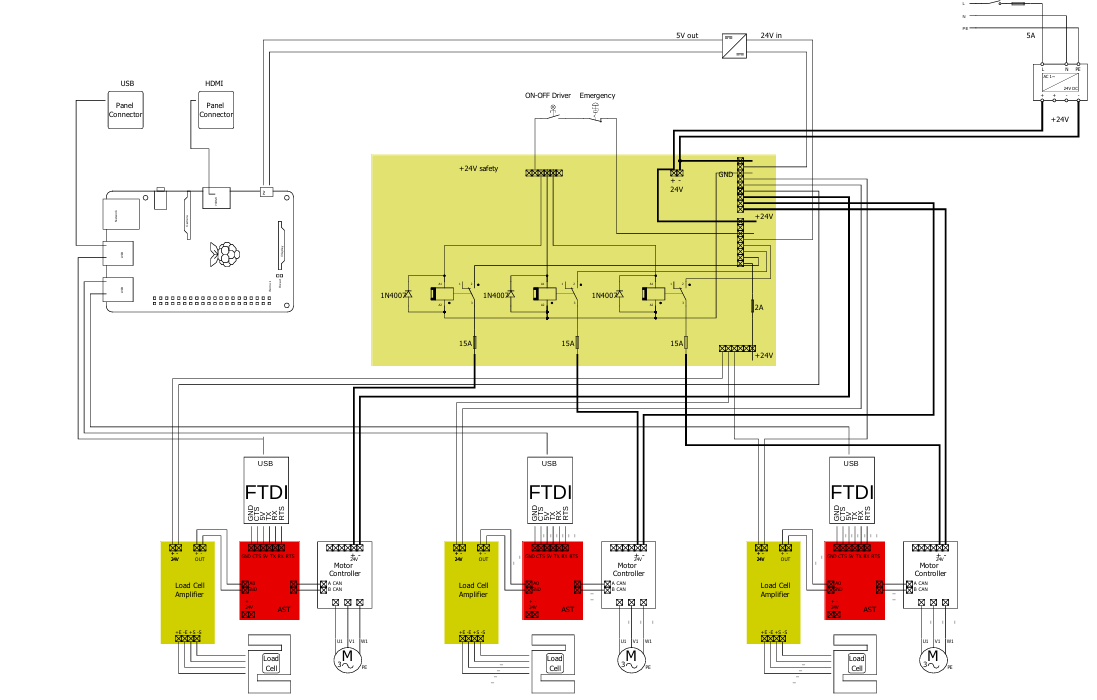
\includegraphics[scale=0.5]{images/chapter7/multifilare.png}
    \caption{Wiring Schematic}
\end{figure}
\FloatBarrier

The computing infrastructure consists of a Raspberry Pi 4 single-board computer, powered by a dedicated DC-DC converter providing a regulated 5 V rail from the 24 V bus. The Raspberry Pi communicates with the three AST-Shield boards through RS232-to-USB adapters, one per channel, connected to its USB ports. The 24 V power bus is supplied by a DIN-rail-mounted HRPG-1000-24 AC-DC converter (Mean Well, 1000 W, 24 V / 41.7 A), which provides sufficient headroom for the three motors operating simultaneously at peak current.

The 24 V power line is distributed to each channel through protection diodes (1N4007, rated 15 A per channel for the motor driver, and 5 A for the load cell amplifier), which prevent cross-channel current injection in the event of a driver fault. An emergency stop circuit, wired in series with the 24 V safety rail, allows the operator to cut power to all motor drivers simultaneously while maintaining the logic supply to the Raspberry Pi and the AST-Shield boards.

\section{Actuator: HT1225 Brushless DC Motor}
The actuator selected for each finger channel is the HT1225 brushless DC motor, a compact gimbal-type PMSM/BLDC unit with integrated slip ring and magnetic encoder. The principal specifications extracted from the manufacturer datasheet are summarised in Table 6.1.

\begin{table}[h]
    \centering
    \begin{tabular}{|c|c|c|}
        \hline
        Parameter & Value & Units \\
        \hline
        Rated Voltage & 24 & V \\
        Rated Current & 4 & A \\
        Rated Torque & 6 & Nm \\
        Rated Speed & 140 & rpm \\
        Maximum No-Load Speed & 300 & rpm \\
        Stall Torque & 6.9 & Nm \\
        Stall Current & 11.2 & A \\
        Phase-to-Phase Resistance & 2.5 & $\Omega$ \\
        Phase-to-Phase Inductance & 66 & mH \\
        Speed Constant & 12 & rpm/V \\
        Torque Constant & 0.76 & Nm/A \\
        Rotor Inertia & 4656 & $g cm^2$ \\
        Pole Pairs & 21 &$ -$ \\
        Motor Weight & 1.3 & kg \\
        Recommended motor load & 25 & kg \\
        Working Temperature Range & -20 to 80 & °C \\
        Encoder Type & AS5048A & - \\
        Encoder Resolution & 14 & bits \\
        Slip ring & 22 & mm \\
        \hline
    \end{tabular}
    \caption{HT1225 Motor Specifications}
\end{table}

The motor's low nominal speed (140 rpm) and high torque-to-weight ratio make it particularly suitable for direct-drive finger actuation without the need for a gearbox, which would introduce backlash and additional compliance. The stall current of 11.2 A exceeds the rated working current of the HT-PTZ driver (7.5 A), which therefore acts as the limiting element in peak torque delivery. At 7.5 A, the estimated peak torque output is approximately 5.7 N·m (using $K_t = 0.76 Nm/A$), which is sufficient for the intended rehabilitation forces.
The integrated AS5048A encoder provides 14-bit absolute position measurement over a full revolution, corresponding to a resolution of 16384 counts/revolution. This value is the effective counts-per-revolution (CPR) used in the BoardClient software for converting raw position counts to angular displacement in degrees. The slip ring allows continuous rotation without cable wrap-up, which is important for exercises requiring multi-turn wrist or finger movements.

\section{Motor Driver: HT-PTZ with AST-CAN485 Interface}
The motor driver used in the prototype is the HT-PTZ magnetic encoder servo drive, a compact field-oriented control (FOC) board designed for brushless PMSM and BLDC motors. The driver implements a cascaded PID control structure with an inner current loop, a speed loop, and an optional outer position loop, all operating on the encoder feedback from the AS5048A sensor connected via SPI.

\subsection{Driver Specifications}
The driver accepts a supply voltage in the range 9-36 V DC (nominal 24 V) and supports working currents up to 7.5 A continuous, with instantaneous overcurrent protection at 20 A implemented in the driver chip. The supported encoder types include the AMS AS5048A (14-bit, 16384 counts/revolution) and the TLE5012B (15-bit, 32768 counts/revolution). The prototype uses the AS5048A variant throughout.
Communication with the host computer is provided through five interface options: USB serial port (via a Silicon Labs CP210x bridge, 115200 baud, 8N1), RS-485 bus (selectable via DIP switch, electrically equivalent to the USB serial protocol), CAN bus (CanOpen protocol, CIA402 dictionary), pulse/direction optocoupler input, and two hardware limit switch inputs. In the prototype, the RS-485 interface is used for all three channels, bridged to USB through RS232-to-USB adapters connected to the Raspberry Pi, enabling reliable long-distance transmission and multi-drop wiring within the electronics enclosure.
The DIP switch on each driver board is configured with bits 1 and 2 in the ON position to activate the RS-485 mode and enable the 120 $\Omega$ termination resistor at the physical end of the bus. Bit 3, controlling the CAN bus termination, is left OFF as the CAN interface is not used in the current implementation.

\subsection{Serial Communication Protocol}
The serial communication protocol used by the HT-PTZ driver follows a text-based line-oriented format at the application level. All commands are ASCII strings terminated by a newline character (\\n). The driver acknowledges each command with either the string OK or an error response prefixed with ERR,. At the lower level, the driver firmware appends a CRC16 checksum to each frame to detect transmission errors.
The telemetry stream, which the driver publishes asynchronously at a configurable rate, adopts the following comma-separated format:

\begin{minted}{bash}

    TEL,<ms>,<force_N>,<angle_deg>,<pos_counts>,<vel_counts_s>,<current_A>

\end{minted}

where \textit{ms} is the driver's internal millisecond timestamp, \textit{force\_N} is the force reading from the load cell amplifier connected to the analogue \textit{input A0}, \textit{angle\_deg} is the absolute angular position converted to degrees by the driver firmware, \textit{pos\_counts} is the raw encoder position in counts, \textit{vel\_counts\_s} is the estimated angular velocity in counts per second (or NaN if unavailable), and \textit{current\_A} is the motor phase current estimate. 

The three high-level commands relevant to the prototype operation are \textit{PING} (connectivity check), \textit{SPD,<deg\_per\_s>} (set speed setpoint in degrees per second), and \textit{STOP} (decelerate to zero and hold position).

\section{Sensing: Load Cell and Finger Encoder}
\subsection{Load Cell and Amplifier}
Each finger is equipped with a strain-gauge load cell mounted at the fingertip contact point. The load cell is wired in a four-wire configuration (excitation +/-, signal +/-) to a dedicated analogue amplifier board, powered from the 24 V bus. The amplifier provides a ratiometric $0-5 V$ output proportional to the applied force, which is connected to the analogue input A0 of the corresponding AST-Shield board. The AST-Shield reads this voltage via its onboard ADC and includes the converted force value in each TEL message, providing force feedback to the Raspberry Pi at the telemetry update rate.
The wiring from the load cell to the amplifier uses the colour convention documented in the shield wiring schematic: the excitation lines connect to the E+ and E- terminals, the signal lines to S+ and S-, and the amplifier output to V and P-. The schematic notes a colour ambiguity on the green/white signal pair that was resolved during assembly through continuity testing. The amplifier ground is shared with the AST-Shield digital ground to avoid common-mode noise on the analogue measurement.

\begin{figure}[ht]
    \centering
    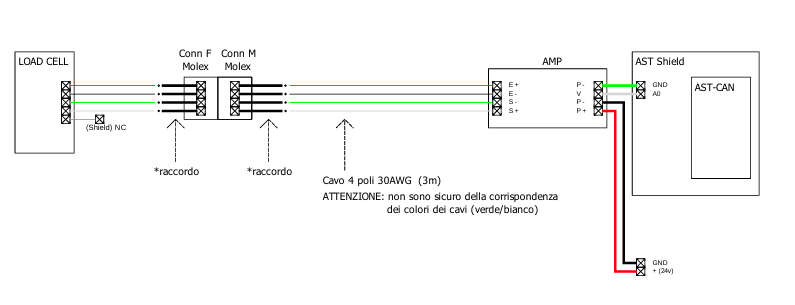
\includegraphics[scale=0.6]{images/chapter7/loadcell_connection.png}
    \caption{Load Cell Connection}
\end{figure}
\FloatBarrier

\subsection{Finger Encoder}
In addition to the motor shaft encoder, each finger channel includes a secondary magnetic encoder mounted directly on the mechanical joint of the finger mechanism. This encoder provides an independent measurement of the actual joint angle, decoupled from any compliance or backlash in the transmission. In the wiring schematic, this encoder is represented as a 4-wire device connected to the AST-Shield through a 3-metre, 30 AWG, 4-pole cable terminated with Molex connectors at both ends. The four lines carry 5 V power, ground, and two digital data lines (D6/D8, the exact assignment depending on the firmware configuration).
The wiring requires a mechanical splicing adapter at both connector ends to transition the 30 AWG cable diameter of the extension to the 20 AWG wire gauge required by the Molex crimp terminals. This adaptation is common in miniaturised wearable robotics where the cable routing path imposes tight diameter constraints.

\begin{figure}[ht]
    \centering
    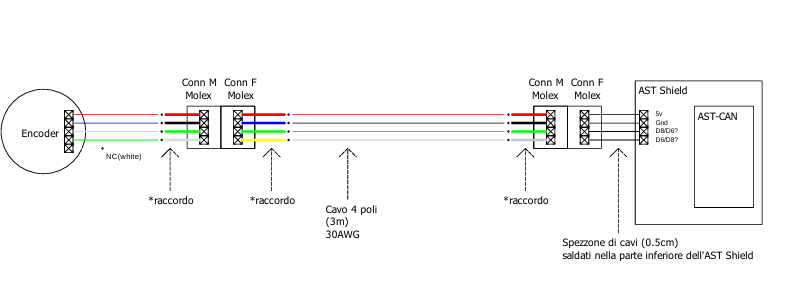
\includegraphics[scale=0.6]{images/chapter7/encoder_connection.png}
    \caption{Finger Encoder Connection}
\end{figure}
\FloatBarrier

\section{Wiring Architecture}
The complete wiring architecture is documented in the multi-wire schematic produced by Humanware. Three structurally identical finger channels are routed in parallel from the panel connector on the enclosure to the individual driver, amplifier, and sensor assemblies on the exoskeleton frame.
Each channel is grounded at a single point through the panel connector to avoid ground loops. The 24 V motor power lines are fused individually: a 15 A diode in series with each motor driver channel limits the maximum sustainable current to a safe value during a fault condition, while the load cell amplifier on each channel is protected by a 5 A diode on its 24 V supply. The RS-485 data pairs from the three AST-Shield boards are routed as independent twisted pairs to the RS232-to-USB adapters on the Raspberry Pi, rather than as a shared RS-485 bus, to avoid the need for address arbitration at the protocol level and to simplify the firmware on the AST-Shield boards.
The FTDI/RS232 converters shown in the multifilare schematic serve as the physical-layer interface between the Raspberry Pi USB ports and the RS-485 differential signal levels on the driver side. The CTS and RTS hardware handshake lines are connected but not actively used in the current firmware, as the telemetry rate is sufficiently low that software flow control is unnecessary at 115200 baud.

\section{Board-Level Software: BoardClient and GUI}
The board-level software comprises two layers: a Python library (BoardClient) that abstracts the serial communication with a single driver board, and a multi-panel Tkinter GUI that wraps three BoardClient instances for simultaneous control of all three finger channels. Both layers were received from Humanware in their original form and subsequently modified to improve reliability and to support the data logging requirements of the digital twin integration.

To support the validation of the digital twin model described in Chapter 4, a data logging capability was developed around the GUI and a suite of offline analysis scripts. The GUI logs all telemetry fields - including the derived position and the commanded speed setpoint at each step - to a CSV file with a mixed schema containing both telemetry rows and event rows. Event rows record GUI actions (Connect, Disconnect, Set Speed, STOP) with the same timestamp as the telemetry rows, enabling precise alignment of command inputs and sensor outputs in post-processing.

The HT-PTZ driver should provide a velocity estimate (vel\_counts\_s) but, at the moment of writing, this field is not populated by the driver firmware and returns NaN. As a workaround, a simple numerical differentiation of the position counts is implemented in the BoardClient library to provide an approximate velocity estimate for analysis purposes. 

The first pipeline (\texttt{estimate\_velocity\_linearfit.py}) applies a local linear regression over a sliding window of half-width \texttt{half\_window} samples centred on each point. For each window, the position samples are fitted to a degree-1 polynomial in time; the slope of the fit is taken as the velocity estimate at the central sample. The time vector can be derived from the monotonic host timestamp (\texttt{t\_mono\_s}) or the driver's internal millisecond counter (\texttt{ms}). NaN samples in the position signal are linearly interpolated before fitting to avoid discontinuities. The method is robust to occasional missing samples but introduces a latency of \texttt{half\_window} samples, which is acceptable for offline processing.

The second pipeline (\texttt{estimate\_velocity\_savgol.py}) applies the Savitzky--Golay differentiation filter, which simultaneously smooths the signal and computes its derivative in a single matrix operation. The filter order and window length are configurable (defaults: order 3, window 31 samples). The median inter-sample interval is used as the filter's \texttt{delta} parameter. To avoid the well-known edge artefacts of the Savitzky--Golay filter, the first and last \texttt{half\_window} samples of the output are set to NaN and excluded from downstream processing. The Savitzky--Golay estimator provides smoother velocity traces than the linear fit at the cost of a longer effective window and a slightly higher computational load, making it the preferred option for kinematic analysis.

The analysis script (analysis.py) loads one or more logged CSV files, separates telemetry rows from event rows, applies optional IQR-based spike rejection on the measured channels (force, angle, position, velocity), and generates a multi-panel time-series plot for each file. Event rows are overlaid on the plots as vertical lines colour-coded by event type: Set Speed events are rendered in bright green (solid, 1.6 pt) and STOP events in red (solid, 2.2 pt), providing an immediately legible view of the command sequence in relation to the sensor signals.

The spike rejection algorithm computes the first and third quartiles (Q1, Q3) of each channel and replaces samples outside the interval [Q1 - k·IQR, Q3 + k·IQR] with NaN, where k is a configurable multiplier (default k = 5). The conservative default is intended to remove only physically implausible outliers (typically arising from ADC transients during a power-on or serial reconnection event) while preserving legitimate signal excursions during rapid motion.

\section{WebSocket-Based Distributed Control}

The \texttt{finger\_client.py} module, provided by the industrial partner, implements a more advanced distributed control architecture intended for deployment scenarios in which the Raspberry Pi on the exoskeleton and the ROS~2 workstation running the digital twin are physically separated. Each finger is managed by an independent \texttt{FingerProcess} instance that maintains its own serial connection to the corresponding HT-PTZ driver and connects to a WebSocket server running on the remote workstation.

The \texttt{FingerProcess} class uses Python's \texttt{asyncio} event loop to multiplex three concurrent coroutines: a WebSocket receiver (\texttt{\_ws\_receiver}) that dispatches incoming command messages, a telemetry sender (\texttt{\_ws\_telemetry\_sender}) that forwards the latest sample from the serial stream to the server at a configurable rate (default 50~Hz), and a serial watchdog (\texttt{\_serial\_watchdog}) that monitors the age of the last received telemetry packet and triggers a serial reconnection if the stream becomes stale. The \texttt{BoardClient} serial callbacks are bridged to the \texttt{asyncio} queue via \texttt{loop.call\_soon\_threadsafe}, preserving thread safety between the serial RX thread and the event loop.

This system decouples the serial polling rate (determined by the driver firmware, typically 100--200~Hz) from the WebSocket transmission rate, enabling bandwidth efficient operation over a standard Wi-Fi or Ethernet link. The per-finger configuration (serial port, baud rate, WebSocket URL, telemetry rate, watchdog timeout) is loaded from JSON files stored in a \texttt{configs/} directory, one file per finger, making the deployment easily reconfigurable without modifying the source code.

\section{Summary}
This chapter has presented the hardware prototype of the Exoskeletron hand exoskeleton, covering the complete electromechanical, electrical, and software stack from the power distribution level to the board-level communication interface. The prototype employs three HT1225 brushless DC motors actuating one finger each, controlled by HT-PTZ field-oriented drive boards communicating over RS-485 at 115200 baud. Force feedback is provided by individual load cell amplifiers at each fingertip, and absolute joint position is available from both the motor shaft encoder (AS5048A, 14-bit) and a secondary finger-mounted encoder.

The board-level Python software was substantially modified with respect to the OEM baseline to introduce a robust auto-reconnection mechanism with stale-RX watchdog, thread-safe GUI updates via a producer-consumer queue pattern, and derived position and velocity computation. Two complementary offline velocity estimation methods — local linear regression and Savitzky-Golay differentiation — were developed to replace the unreliable firmware velocity estimate at low speeds, providing clean kinematic signals suitable for comparison with the digital twin model outputs.

The hardware architecture described in this chapter constitutes the physical counterpart of the digital twin: the signal channels, sensor types, communication latencies, and actuation dynamics documented here are the reference against which the simulation model of Chapter 4 was calibrated, and they define the interface requirements that a future hardware-in-the-loop integration of the ROS2 stack with the physical prototype will need to satisfy.










